\section{Dependency Graph}
A Dependency Graph is a graphical representation of the which module is dependent on which other modules. A Dependency Graph is often used as a preliminary step to creating an overview of the system. Dependency Graph also gives overview of how good is the design of the system.
OpenSCAD being were huge software it would be difficult to make the dependency graph of whole software. So, here is  Dependency Graph of Customizer is as following-:
\begin{enumerate}
\item \textbf{Dependency graph of Comment.h:} Figure \ref{fig:comment1} shows the modules on which the comment.h module is dependent.
\item \textbf{Caller graph of Comment.h:} Figure \ref{fig:comment} shows the modules that use the module comment.h.
\item \textbf{Caller graph of ParameterWidget.cc:} Figure \ref{fig:dependency} show the modules that uses the module ParameterWidget.h.
\end{enumerate}

\begin{figure}
	\centering
	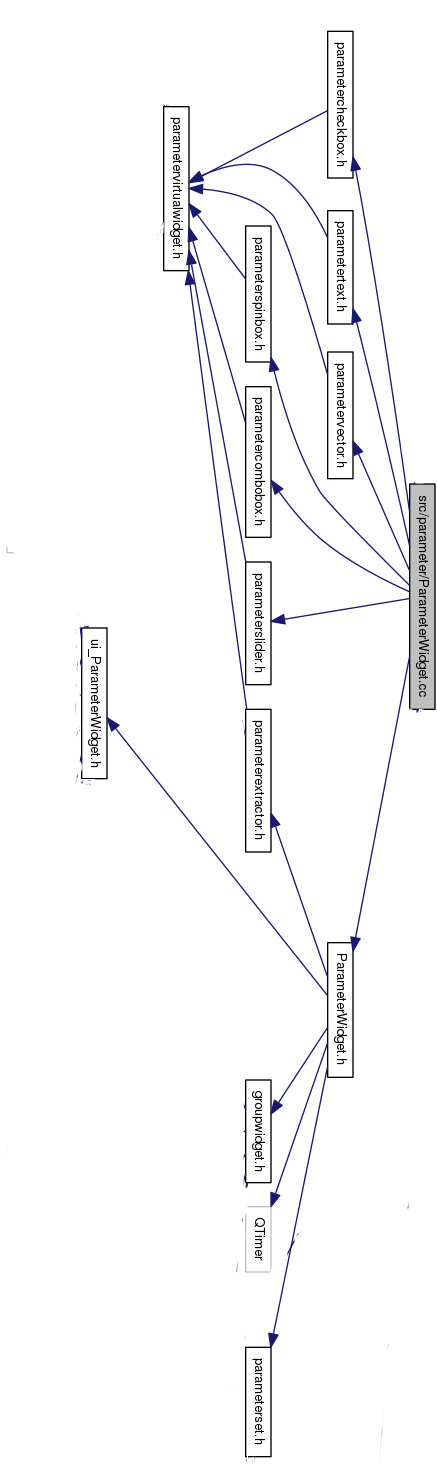
\includegraphics[width=0.7\linewidth,height=1.37\columnwidth]{images/dependene}
	\caption{ Dependency graph of Comment.h}
	\label{fig:dependency}
\end{figure}

\begin{figure}
\centering
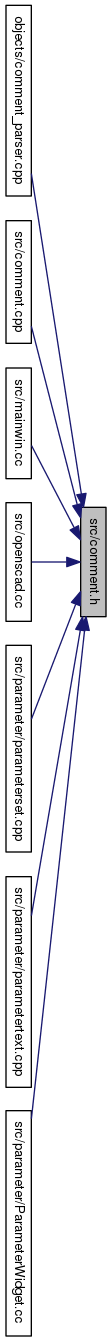
\includegraphics[width=0.25\linewidth,height=1.37\columnwidth]{images/comment}
\caption{Caller graph of Comment.h}
\label{fig:comment}
\end{figure}
\begin{figure}
\centering
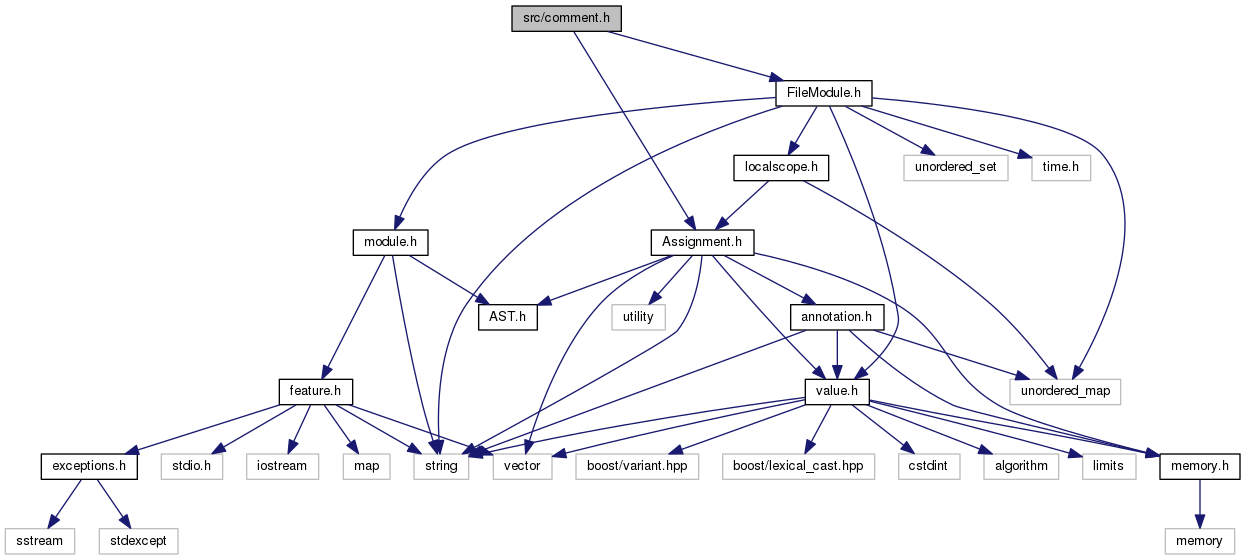
\includegraphics[width=\linewidth,height=1.35\columnwidth]{images/comment1}
\caption{Caller graph of ParameterWidget.cc}
\label{fig:comment1}
\end{figure}


\section{Flowchart}
A flowchart is a type of diagram that represents an algorithm, work flow or process, showing the steps as boxes of various kinds, and their order by connecting them with arrows
and the flowchart \ref{fig:FD1} of customizer showing the flow of control and Data in the software.

\begin{figure}
    \centering 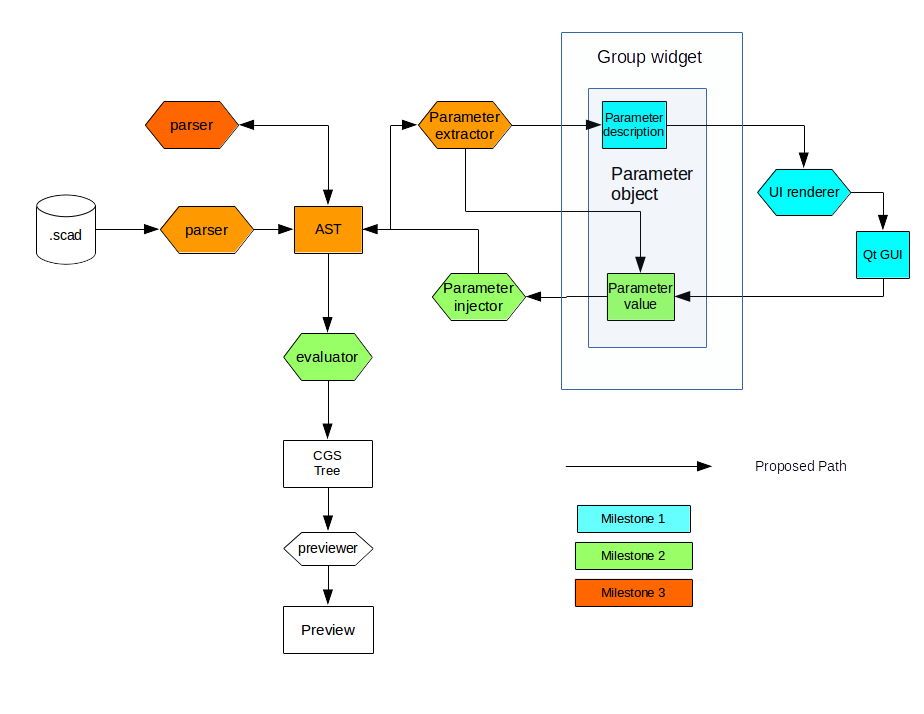
\includegraphics[scale=0.65]{images/flowchart.png}
    \caption{Flowchart of Customizer}
    \label{fig:FD1}
\end{figure}

\subsection{Detailed Description}

The basic implementation of this project is almost done in form of prototype. There is need to modify the structure of the project. We have to divide the task into there parts:

\begin{enumerate}
    \item \textbf{Front end}
    It will deal with how the parameter will look to the user like in form of range or spinbox etc. This part will include two parts:
    \begin{enumerate}
        \item \textbf{Individual Parameter}
        This will define how individual parameters will look like
        \item \textbf{Container Widget}
        This will contain UI features common to all parameter. This widget will contain all parameter widget.
       
    \end{enumerate}
   
    \item \textbf{Back End}
    This will include the parser part that will create AST nodes and we can extract the parameters from the AST. we can use the single parser for the whole .scad file or separate parser for extracting the parameters with annotations.
   
    The Back-end part will also include the parameter extractor and injector or the injector can be included in parameter object which will serve as interface
    \item \textbf{Interface}
    This will include the parameter object which will serve as an interface between both Back end and Front end. Parameter object will contain information regarding each individual parameter like parameter name, default value, and information how this parameter will be displayed as widgets to the user. Parameter object could also include the method to inject the value of the individual parameter into the AST.
   
\end{enumerate}

\section{Class Diagrams}
Class Diagrams describe the static structure of the system. Following classes diagram represent the relationship between different classes in OpenSCAD and customizer:
\begin{enumerate}
	\item Figure \ref{fig:collaborative1} shows the class diagram of the ParameterWidgetVirtual class which is the basse class of all the Widget classes i.e ParameterCheckbox, ParameterVector,ParmeterSpinbox, ParameterComboBox,ParameterSlider, ParameterText.
	\item Figure \ref{fig:collaborative} shows the class diagram of the ParameterWidget class which is the main class for whole the Customizer GUI and also show how this class is related to various classes in custmoizer.
	
	\item Figure \ref{fig:classAnnotation__coll__graph}  shows the class diagram of the Annotation class which is the main node of the AST that support the customizer feature and also show how this class is related to various classes in the customizer.
\end{enumerate}
\begin{figure}
    \centering
    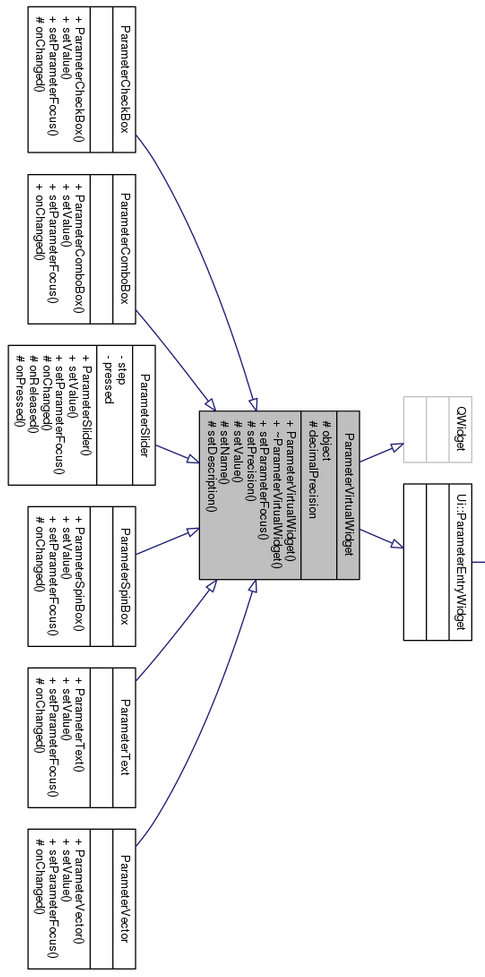
\includegraphics[width=0.5\linewidth,,height=1.38\columnwidth]{images/collaborative1}
    \caption{Class Diagram for Customizer (Part A) }
    \label{fig:collaborative1}
\end{figure}
\begin{figure}
    \centering
    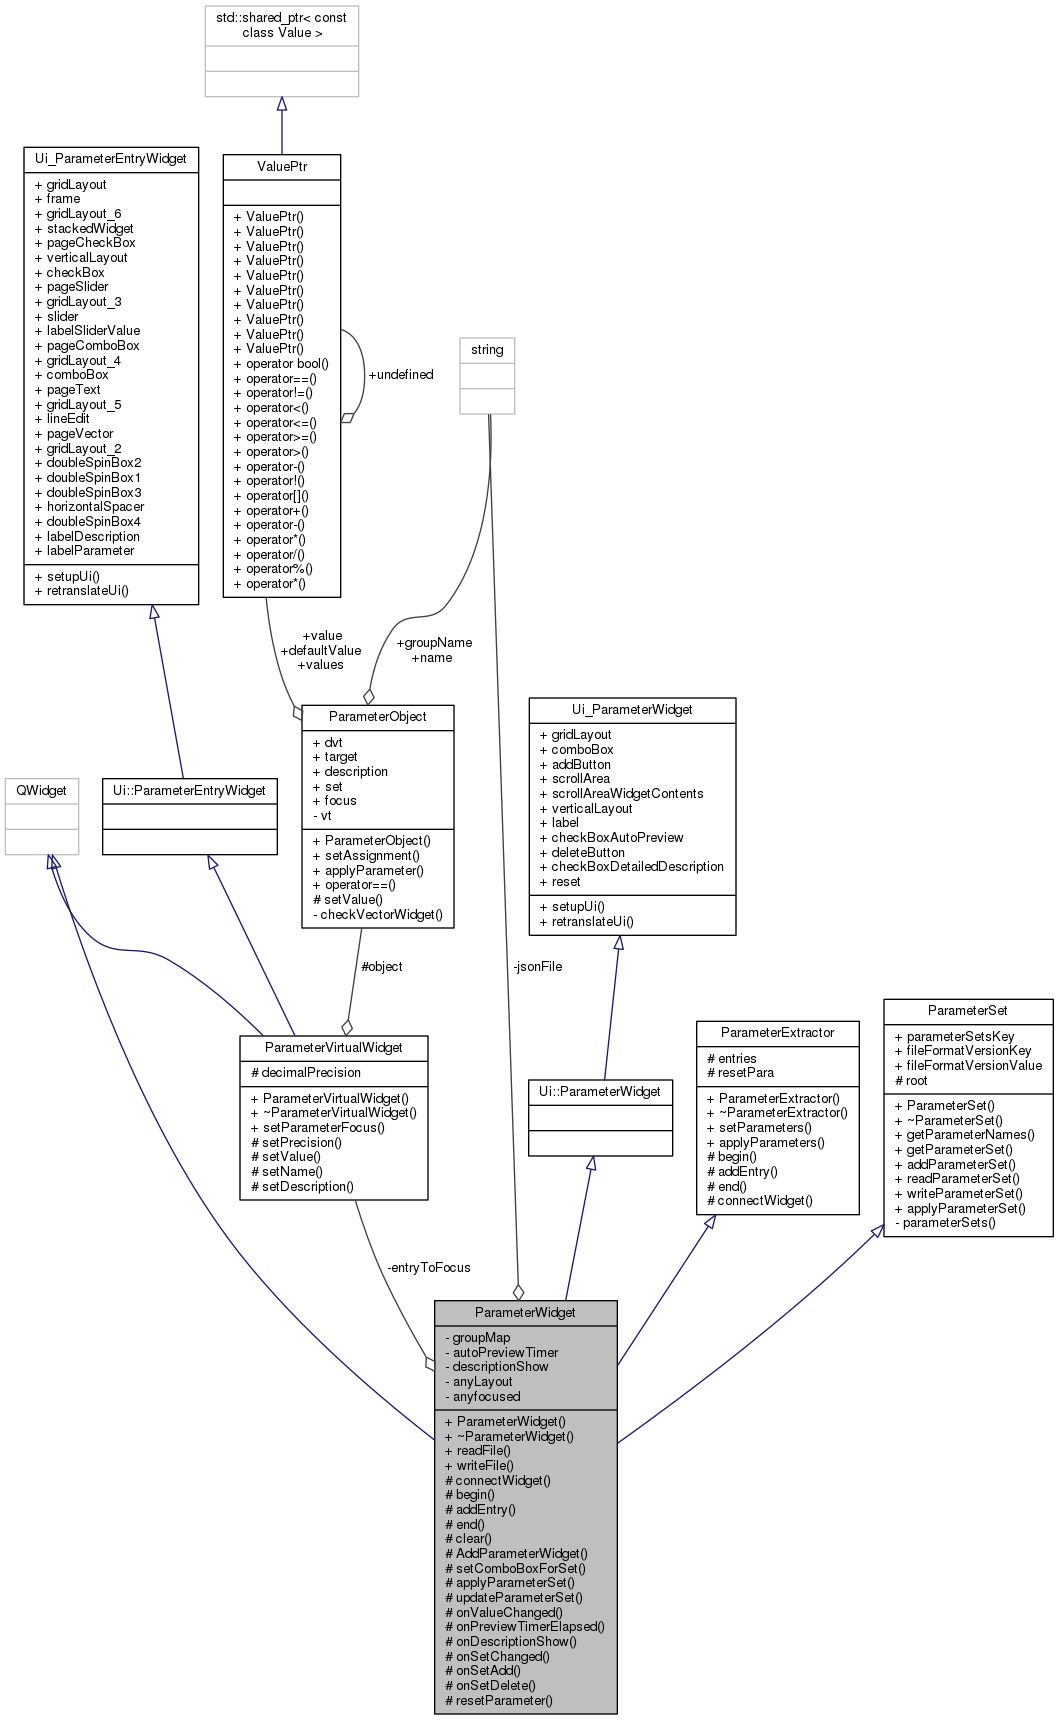
\includegraphics[scale=0.40]{images/collaborative}
    \caption{Class Diagram for Customizer (Part B)}
    \label{fig:collaborative}
\end{figure}
\begin{figure}
\centering
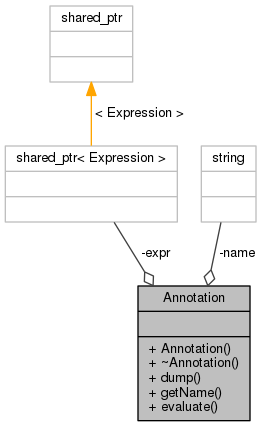
\includegraphics[width=0.4\linewidth]{images/classAnnotation__coll__graph}
\caption{Class Diagram for Annotation}
\label{fig:classAnnotation__coll__graph}
\end{figure}